\documentclass[twoside,11pt]{homework}
\usepackage{listings}
\usepackage{xcolor}
\usepackage{graphicx} 
\setlength{\parskip}{1em}
\renewcommand{\baselinestretch}{1.5}
\usepackage{hyperref}

\coursename{COMS 4771 FALL18} 

\studname{Amal Alabdulkarim (aa4235), Ruolin Jia (rj2537), Jing Qian (jq2282)}    % YOUR NAME GOES HERE
%\studmail{jq2282@columbia.edu}% YOUR UNI GOES HERE
\hwNo{1}                   % THE HOMEWORK NUMBER GOES HERE
\date{\today} % DATE GOES HERE


\begin{document}
\maketitle

\section*{Problem 1}
\subsection*{i)}
Let $x_{min}$ be the smallest element in our samples $X$. Let $x_{max}$ be the maximal element in $X$. 
Let $f(x;a,b)$ be the density function parameterized by $a$ and $b$.
The likelihood can be written as
\begin{equation}
    L(a,b|X) = \prod_{i=1}^n f(x_i)
\end{equation}

\noindent \textbf{Lemma 1:} For any $X$, if parameters $a > x_{min}$ or $b < x_{max}$, then $L(a,b|X)=0$. \\
\textbf{Lemma 1 Proof}: \\
Assume $a > x_{min}$, then $f(x_{min}) = 0$ by the definition of our density. $f(x_{min})$ is a factor in $L(a,b|X)$. Therefore, $L(a,b|X) = 0$. \\
Assume $b < x_{max}$, then $f(x_{max}) = 0$ by the definition of our density. $f(x_{max})$ is a factor in $L(a,b|X)$. Therefore, $L(a,b|X) = 0$. \\

\noindent \textbf{Lemma 2:} For any $X$, if parameters $a <= x_{min}$ and $b >= x_{max}$, then $L(a,b|X) > 0$. \\
\textbf{Lemma 2 Proof}: \\
By definition of our density, $f(x) \propto 1$ when $a \leq x \leq b$. By the definition of ``proportional", it means that there is a constant $k$ s.t. $k>0$ and $f(x) = k$ when $a \leq x \leq b$. 
Therefore, for any $x \in X$ s.t. $a \leq x \leq b$, $f(x) > 0 $. 

If $a \leq x_{min}$ and $b \geq x_{max}$, then all $x \in X$ satisfy $a \leq x \leq b$. Therefore, all factors $f(x_i)>0$ in $L(a,b|X)$. So $L(a,b|X)>0$. 

Let $a_1 \leq x_{min}$ and let $b_1 \geq x_{max}$ and $a_1, b_1$ be the parameters of $L(a_1, b_1|X)$. Let $a_2 > x_{min}$ or $b_2 < x_{max}$ and $a_2, b_2$ be the parameters of $L(a_2, b_2|X)$. 


With \textbf{Lemma 1} and \textbf{Lemma 2}, $L(a_1, b_1|X) > L(a_2, b_2|X)$. Therefore, the MLE, if it exists, of $a$ and $b$ must satisfy $a_1 \leq x_{min}$ and $b_1 \geq x_{max}$. Now, to find MLE of $a$ and $b$, we don't need to consider the range $(x_{min}, x_{max})$.
\\
\noindent Let $b \leq x_{max}$ and $a \geq  x_{min}$. We know that there is a constant $k$ s.t. $k>0$ and $f(x) = k$ when $a \leq x \leq b$. $f(x)$ is a density so $\int_{-\infty}^{\infty}f(x)dx = 1$. Since, $f(x) = 0$ when $ x < a$ or $x > b$, then $\int_{a}^{b}f(x)dx = 1$. Since $a \leq x \leq b$, we have $\int_{a}^{b}kdx = 1$. Evaluate this integral, we have $(b-a)k = 1$. Therefore, $k = \frac{1}{b-a}$. Therefore, for $x$ s.t. $a \leq x \leq b$, $f(x) = \frac{1}{b-a}$. 

Since $a \leq x_{min}$ and $b \geq x_{max}$, all $x$ in our dataset satisfy $a \leq x \leq b$. Our likelihood can be written as:

\begin{align*}
    L(a,b|X) &= \prod_{i=1}^n f(x_i) \\
    				&= \prod_{i=1}^n \frac{1}{b-a} \\
                    &= \frac{n}{b-a}
\end{align*}
Let $a \geq x_{min}$ and $b \leq x_{max}$ hold. Let $a'$ be a real value s.t. $a'<a$. We get the inequality: 

\begin{align*}
\frac{n}{b-a} >&\frac{n}{b-a'}  \\
\end{align*}
Therefore, 

\begin{align*}
L(a,b|X)  >& L(a,b'|X)   \\
\end{align*}

Similarly, let $b'$ be a real value s.t. $b'>b$, We know that
\begin{align*}
\frac{n}{b-a} > &\frac{n}{b'-a}  \\
\end{align*}
Therefore,
\begin{align*}
L(a,b'|X)  <& L(a,b|X)   \\
\end{align*}
We have shown that the MLE of $a$ and $b$ cannot be in the range $(x_{min}, x_{max})$ because it will result in zero likelihood. From the above derivation, if we fix $b$, we know that a greater $a$ will result in a greater $L(a, b)$. If we fix $a$,  a smaller $b$ will result in a greater $L(a,b|X) $. Therefore $a=x_{min}$ and $b=x_{max}$ will maximize $L(a,b|X)$, Therefore, the MLE of $a$  is $x_{min}$ and the MLE of $b$ is $x_{max}$. 

\newpage
\subsection*{ii)}

Firstly, this rule can be proved by using supremum, which is a state-of-art proof in some text books. This proof can be found in this link \footnote{\url{http://www.stat.unc.edu/faculty/cji/lecture7.pdf}}. 

We can cite this theorem to solve this problem. However, since directly citing this proof or applying this proof will make this problem trivial, we decide to solve the problem by deriving our own way.

Let $g(\theta)$ be a continuous many-to-one function and $g(\theta) = t$.

Let the likelihood function parameterized by $\theta$ be:

\begin{equation*}
    L_{1}(\theta|X)
\end{equation*}Then, with the same $X$ and $\theta$, there are a set of likelihood functions $L_{2}^{i}(t|X)$ where $i = 1...n$ (n can be $\infty$) parameterized by $t$ such that $g(\theta) =t$. These likelihood functions are transformed from $L_{1}(\theta|X)$ and there is no change on the data and density function during the transformation. Therefore, $L_{2}^{i}(t|X) = L_{1}(\theta|X)$ for all $i$ . We call this set of functions as transformed likelihoods of $L_{1}(\theta|X)$. 

Let the domain of $L_{1}(\theta|X)$ be $\Theta$. Let the domain of a transformed likelihood $L_{2}^{i}(t|X)$  be $T_i$. 

\noindent \textbf{Lemma 1: } For any transformed likelihood $L_{2}^{i}(t|X)$ and any $t \in T_i$, there exists some $\theta_{t} \in \Theta$, such that $g(\theta_{t}) = t$ and  $L_{1}(\theta_t|X) = L_{2}^{i}(t|X)$. \\
\noindent \textbf{Lemma 1 proof: } For all $i$, any likelihood value of $L_{2}^{i}(t|X)$ is transformed from $L_{1}(\theta_t|X)$ for some $\theta_t \in \Theta$ by transforming parameters from $\theta_t$ to $t$ with $g(\theta) = t$, therefore, the lemma holds true. In other words, we can always find a corresponding $L_{1}(\theta_t|X)$ given a $L_{2}^{i}(t|X)$ and the mapping from $\theta_t$ to $t$ is obtained by $g(\theta_t) = t$ . If we cannot find a corresponding $L_{1}(\theta_t|X)$, it means this $L_{2}^{i}(t|X)$ is transformed from nowhere, which means that $L_{2}^{i}(t|X)$ cannot exist. 

We know $\theta_{MLE} = {argmax}_{\theta}~L_{1}(\theta|X)$ by definition. 

Let $g(\theta_{MLE}) = h$ , then the transformed likelihoods of $L_{1}(\theta_{MLE}|X)$ will be $L_2^i(h|X)$,  $i = 1...n$ and $L_{1}(\theta_{MLE}|X) = L_2^i(h|X)$ for all $i$. 

Assume $ h \neq argmax_{t}L_{2}^{i}(t|X)$ for some $i$. Then there exists a $z \in T_i$ such that $L_{2}^{i}(z|X) > L_{2}^{i}(h|X)$. 

By \textbf{Lemma 1}, we know that there exists a $\theta_z$ such that $\theta_{z} \in \Theta$,  $g(\theta_{z}) = z$ and  $L_{1}(\theta_z|X) = L_{2}^{i}(z|X)$. Then $L_{1}(\theta_z|X) > L_{2}^{i}(h|X) \\$. 

Since $L_{1}(\theta_{MLE}|X) = L_2^i(h|X)$, we get $L_{1}(\theta_z|X) > L_{1}(\theta_{MLE}|X) $. This is a contradiction. 

Therefore, $ h = argmax_{t}L_{2}^{i}(t|X)$ for all i. 

We proved $ g(\theta_{MLE}) = argmax_{t}L_{2}^{i}(t|X) = argmax_{g(\theta)}L_{2}^{i}(g(\theta)|X)$ 

\newpage
\subsection*{iii)}
Let $\theta = E(X)$. This is the true value that we want to estimate
\subsubsection*{Consistent and Unbiased}
Example 1:
MLE of $\theta$ is both consistent and unbiased \footnote{\url{https://en.wikipedia.org/wiki/Maximum_likelihood_estimation}}.
To make the explanation easier, we can use $\theta_{MLE}$ as a benchmark estimator. We can show that if an estimator is the same as $\theta_{MLE}$ when $n \to \infty$, then it is consistent. We will to this approach in the rest of this question.
\begin{equation*}
\theta_{MLE}= \frac{1}{n} \sum_{i=1}^{n} x_{i}
\end{equation*}\noindent Example 2:
Take the sample mean of the half of the samples. 
\begin{equation*}
\hat{\theta} = \frac{1}{2n} \sum_{i=1}^{\frac{n}{2}} x_{i}
\end{equation*}It is consistent since when $n \to \infty$, it is the same as MLE of $\theta$ , so it is consistent as MLE of $ \theta$. 

\noindent It is unbiased since $E(\hat{\theta}) = E(\theta_{MLE})$, therefore, since $\theta_{MLE}$ is unbiased , this $\hat{\theta}$ is unbiased.

\subsubsection*{Consistent and Biased}
Example 1:
\begin{equation*}
\hat{\theta} = \frac{n}{n-1}\bar{x}
\end{equation*}
$\bar{x}$ is the sample mean. 
When $n \to \infty$: 
\begin{equation*}
\lim_{n \to \infty} (\frac{n}{n-1}\bar{x}) = E(X) = \lim_{n \to \infty} \theta_{MLE} 
\end{equation*}
\noindent $\hat{\theta}$ will be same as the $\theta_{MLE}$. Since $\theta_{MLE}$ is consistent, then $\hat{\theta}$ is consistent. 
It is biased because:
\begin{equation*}
E[\hat{\theta}] = E[\frac{n}{n-1}\bar{x}] = \frac{n}{n-1}E(X) \neq E[X] = \theta
\end{equation*}


\noindent Example 2:
\noindent $x_1$ is a example from the sample set
\begin{equation*}
\hat{\theta} = \bar{x} + \frac{x_1}{n}
\end{equation*}\noindent  is consistent because
\begin{equation*}
\lim_{n \to \infty} (\bar{x} + \frac{x_1}{n}) = E(X) = \lim_{n \to \infty} \theta_{MLE} 
\end{equation*}
\noindent Similar to Example 1, it is consistent.

\noindent It is biased because: 
\begin{equation*}
E(\hat{\theta}) = E(\bar{x} + \frac{x_1}{n}) = E(X) + \frac{1}{n}E(X) \neq \theta
\end{equation*}
\newpage

\subsubsection*{Inconsistent and Unbiased}
Example 1:
Just use one example from the sample set as the estimator

\begin{equation*}
\hat{\theta} = x_{1}
\end{equation*}
It is inconsistent because when $n \to \infty$, still $\hat{\theta} = x_{1}$. $\hat{\theta}$ is not affected by $n$ so $P(|\hat{\theta}- \theta| \geq \epsilon) \to 0$ does not hold. 
It is unbiased because $E(x_{1}) = E(X) = \theta$. 

Example 2:
Take the average of any two examples from the sample set. 

\begin{equation*}
\hat{\theta} = \frac{x_{1} + x_{2}}{2}
\end{equation*}
It is inconsistent due to the same reason as Example 1. 
But it is unbiased:

\begin{equation*}
\hat{\theta} = \frac{x_{1} + x_{2}}{2} = \frac{1}{2}E(X+X) = E(X) = \theta
\end{equation*}
\subsubsection*{Inconsistent and Biased}
Example 1:
\begin{equation*}
\hat{\theta} = \bar{x} + 1
\end{equation*}

It is biased because $E(\bar{x} + 1) = E(X) + 1 \neq \theta$
It is inconsistent because
\begin{equation*}
\lim_{n \to \infty} \bar{x} + 1 = E(X) + 1
\end{equation*}
This makes $P(|\hat{\theta}- \theta| \geq \epsilon) \to 0$ when $n \to \infty$ false. 
\noindent Example 2:
Take the inverse of one example from the sample. 
\begin{equation*}
\hat{\theta} =  -x_{1}
\end{equation*}It is biased because $E(-x_{1}) = -E(X)  \neq \theta$
It is inconsistent because:
\begin{equation*}
\lim_{n \to \infty}  -x_{1} = -x_{1} 
\end{equation*}This makes $P(|\hat{\theta}- \theta| \geq \epsilon) \to 0$ when $n \to \infty$ false, too. 
\newpage
\section*{Problem 2}
\subsection*{i}
The density of the data distribution can be written as:
\begin{equation*}
f(x;b) = b^{x}(1-b)^{1-x} ~~~where~x \in \{0, 1\}
\end{equation*}
Given the estimator $\hat{b}$, the log likelihood can be written as 
\begin{equation*}
\begin{split}
l(\hat{b}; X) &= \sum_{i=1}^{n} log [\hat{b}^{x_i}  (1-\hat{b})^{1-x_i}] \\
			&=  \sum_{i=1}^{n} x_{i}log\hat{b} + \sum_{i=1}^{n}  (1-x_i) log(1-\hat{b}) \\
            &= \sum_{i=1}^{n} x_i log\hat{b} + nlog(1-\hat{b}) - \sum_{i=1}^{n} x_i log(1-\hat{b})
\end{split}
\end{equation*}
Let
\begin{equation*}
\begin{split}
\frac{\textbf{d}l(\hat{b};X)}{\textbf{d}\hat{b}} &= 0 \\
\sum_{i=1}^{n} \frac{x_i}{\hat{b}} - \frac{n}{1-\hat{b}} + \sum_{i=1}^{n}\frac{x_i}{1-\hat{b}} &= 0 \\
\frac{1}{\hat{b}}\sum_{i=1}^{n} x_i - \frac{1}{1-\hat{b}} (n - \sum_{i=1}^{n} x_i) &= 0 \\
\frac{1}{\hat{b}}\sum_{i=1}^{n} x_i &= \frac{1}{1-\hat{b}} (n - \sum_{i=1}^{n} x_i)  \\
\sum_{i=1}^{n} x_i - \hat{b}\sum_{i=1}^{n} x_i &= \hat{b}n - \hat{b}\sum_{i=1}^{n} x_i \\
\sum_{i=1}^{n} x_i &= \hat{b} n \\
\hat{b} &= \frac{\sum_{i=1}^{n}x_i}{n}
\end{split}
\end{equation*}

To check whether this $\hat{b}$ is a maximizer, we can easily take the second derivative of $l(b; X)$ and check if it is negative. 
\begin{equation*}
\begin{split}
\frac{\textbf{d}^2l(\hat{b};X)}{\textbf{d}\hat{b^2}} &= -\frac{1}{b^2}\sum_{i=1}^{n}x_i - \frac{1}{(1-b)^2} \sum_{i=1}^{n} (1 - x_i)
\end{split}
\end{equation*}

$x_i$ can only be $1$ or $0$. If $x_i = 0$, then $(1-x_i)=1$ and vice versa. Therefore, the second derivative must be negative. 
\newpage

\subsubsection*{ii}
To show consistency, we need to show:
\begin{equation*}
\begin{split}
Pr(|\hat{b} - b| \geq \epsilon)  \to 0 ~~ when~~n \to \infty
\end{split}
\end{equation*}
According to the Law of Large Number \footnote{\url{https://www.dartmouth.edu/~chance/teaching_aids/books_articles/probability_book/Chapter8.pdf}}
\begin{equation*}
\begin{split}
Pr(|\bar{x} - b| \geq \epsilon)  \to 0 ~~ when~~n \to \infty
\end{split}
\end{equation*}
where $\bar{x}$ is the sample mean. In our case, $\bar{x} = \hat{b}$. Therefore, it is consistent

To show it is unbiased: 
\begin{equation*}
\begin{split}
\mathbb{E}[\hat{b}]  &= \mathbb{E}[\frac{\sum_{i=1}^{n}x_i}{n}] \\
									&= \frac{1}{n} \mathbb{E}[nX] = E(X) = b
\end{split}
\end{equation*}
It is unbiased. 
\newpage

\subsubsection*{iii}
%
\begin{equation}
\begin{split}
\mathbb{E} [x] &= \frac{1}{n} \sum_{i=1}^n [1 \times b + 0 \times (1-b)]\\
		      &= \frac{1}{n} \sum_{i=1}^n b \\
		      &= b, \\
\mathbb{E} [x^2 ] 	&= \frac{1}{n} \sum_{i=1}^n [1^2 \times b + 0^2 \times (1-b)]\\
		      &= \frac{1}{n} \sum_{i=1}^n b \\
		      &= b, \\
\mathrm{Var}[x] &= \mathbb{E} [x^2 ] - \mathbb{E} [x]^2 \\
		        &= b - b^2.
\end{split}
\end{equation}
%
\\\\
\subsubsection*{iv}

From subproblem (i), we get the MLE bias $\hat{b} =\frac{\sum_{i=1}^n x_i}{n} $.
From subproblem (ii), we get the variance of this coin is $\mathrm{Var}[x] = b - b^2$.
By applying the invariance property of MLE shown in Problem 1(ii), the MLE for the coin's variance is :
%
\begin{equation}
\hat{\mathrm{Var}}[x] = \hat{b}- \hat{b}^2 = \frac{\sum_{i=1}^n x_i}{n} - (\frac{\sum_{i=1}^n x_i}{n})^2.
\end{equation}

\newpage
\subsubsection*{v}
By applying Bayes Rule, we can get the posterior:

\begin{equation*}
\begin{split}
Post(b|X) = \frac{P(X|b)P(b)} {P(X)}
\end{split}
\end{equation*}
\newpage
We want: 
\begin{equation*}
\begin{split}
\hat{b} = argmax_{b}~Post(b|X) = argmax_{b}~\frac{P(X|b)P(b)} {P(X)}
\end{split}
\end{equation*}
It is equivalent to:
\begin{equation*}
\begin{split}
\hat{b} = argmax_{b}~Post(b|X) = argmax_{b}~P(X|b)P(b)
\end{split}
\end{equation*}
With data express $P(X|b)P(b)$ as a function of $b$, written as $L_{MAP}(b|X)$:

\begin{equation*}
\begin{split}
L_{MAP}(b|X)  &= \prod_{i=1}^{n}[b_{x_i}(1-b)^{1-x_i}]P(b)
\end{split}
\end{equation*}
We can take the log of this  $L_{MAP}(b|X)$ and optimize it by finding a $b$. It will give us the same $\hat{b}$:
\begin{equation*}
\begin{split}
l_{MAP}(b|X)  &= \sum_{i=1}^{n}[\log(b_{x_i}(1-b)^{1-x_i})] + \log(P(b)) \\
							&= \log b \sum_{i=1}^{n} x_i + n\log (1-b) - \log (1-b) \sum_{i=1}^{n} + \log 2b
\end{split}
\end{equation*}
Take the first derivative of $l_{MAP}(b|X)$ with respect to $b$. Let the derivative be $0$ and solve $b$
\begin{equation*}
\begin{split}
\frac{\textbf{d} l_{MAP}(b|X)}{\textbf{d} b} = \frac{1}{b} \sum_{i=1}^{n} x_i  - \frac{n}{1-b} + \frac{1}{1-b}\sum_{i=1}^{n} x_i + \frac{1}{b} &= 0 \\
\frac{1}{b}(\sum_{i=1}^{n} x_i  + 1) & = \frac{1}{1-b}(n - \sum_{i=1}^{n} x_i) \\
b + bn &= \sum_{i=1}^{n} x_i  + 1 \\
b &= \frac{\sum_{i=1}^{n} x_i  + 1}{n+1}
\end{split}
\end{equation*}
We check its second derivative to ensure it is a maximal point: 
\begin{equation*}
\begin{split}
\frac{\textbf{d}^2 l_{MAP}(b|X)}{\textbf{d} b^2} &=  -\frac{1}{b^2}\sum_{i=1}^{n} x_i - \frac{n}{(1-b)^2} + \frac{1}{(1-b)^2}\sum_{i=1}^{n} x_i - \frac{1}{b^2}\\
&= -\frac{1}{b^2}(\sum_{i=1}^{n} x_i + 1) - \frac{1}{(1-b)^2}(n-\sum_{i=1}^{n} x_i)
\end{split}
\end{equation*}
Since $x_i$ can only take $0$ or $1$,  $\sum_{i=1}^{n} x_i + 1 > 0 $ and $(n-\sum_{i=1}^{n} x_i) \geq 0$. The whole expression must be smaller than 0. Therefore, the $b$ we found is a maximizer. In summary:
\begin{equation*}
\begin{split}
\hat{b} = \frac{\sum_{i=1}^{n} x_i  + 1}{n+1}
\end{split}
\end{equation*}


\newpage
%%%%%%%%%%%%%
\subsubsection*{vi}
In general, when $b$ has a uniform distribution, MAP estimate equals MLE.
In other words, $P(b)=k$ where $k$ is a constant.  

From the definition, the MLE and MAP estimations of parameter $b$ are:
\begin{equation}
\begin{split}
b_{\mathrm{MLE}} &= \mathrm{arg\ max}_b \prod_{i=1}^N P(\overrightarrow{x_i}|b) \\
			   &= \mathrm{arg\ max}_b \sum_{i=1}^N \log P(\overrightarrow{x_i}|b) , \\
b_{\mathrm{MAP}} &= \mathrm{arg\ max}_b \prod_{i=1}^N P(b|\overrightarrow{x_i}) \\
                                   & = \mathrm{arg\ max}_b \prod_{i=1}^N P(\overrightarrow{x_i}|b) P(b) \\
                                   &= \mathrm{arg\ max}_b (\log P(b) + \sum_{i=1}^N \log P(\overrightarrow{x_i}|b)).
\end{split}
\end{equation}To maximize MLE and MAP we need to take the derivative to find the optimal point.
$(\log P(b) + \sum_{i=1}^N \log P(\overrightarrow{x_i}|b))$ and $\sum_{i=1}^N \log P(\overrightarrow{x_i}|b)$ have the same derivative given that $\log P(b) $ is a constant. Therefore, MAP and MLE will be the same. 

Also, if by any chance all observations equal to $1$, then MLE and MAP will have the same estimated value regardless of the distribution of $b$. 

Following are the MLE of $b$ from question (i) and MAP estimation of $b$ from question (v):
\begin{equation}
\begin{split}
b_\mathrm{MAP}  &= \frac{\sum_{i=1}^{n} x_i  + 1}{n+1} \\ %= \frac{n+1}{n+1} = 1 \\
b_\mathrm{MLE} &= \frac{\sum_{i=1}^{n} x_i}{n} %= \frac{n}{n} = 1
\end{split}
\end{equation}
When $b_\mathrm{MAP} = b_\mathrm{MLE}$, we have:
\begin{equation}
\begin{split}
b_\mathrm{MAP} &= b_\mathrm{MLE} \\
\frac{\sum_{i=1}^{n} x_i  + 1}{n+1} &= \frac{\sum_{i=1}^{n} x_i}{n} \\
\sum_{i=1}^{n} x_i &= n
\end{split}
\end{equation}
Since $x_i$ could only be 0 or 1, $\sum_{i=1}^{n} x_i = n$ if and only if $x_i = 1$ for every $i$ from i to $n$.

In conclusion, for the general case, MAP estimate equals MLE when parameter $b$ has a uniform distribution. Or in a special case, if all observations equal to $1$, then MLE and MAP will have the same estimated value regardless of the distribution of $b$. 
\newpage
\section*{Problem 3}
\subsection*{i)}
\begin{equation}
\begin{split}
Q(g) = \mathbb{E}_{x,y}[(g(x) - y)^{2}] 
\end{split}
\end{equation}
Let $Q(g)$  be the quality of $g$ and $Q(f)$
be the quality of $f$. We have to show that for any g: 
\begin{equation}
\begin{split}
Q(f)\leq Q(g)
\end{split}
\end{equation}
Proof:  \\
\begin{equation}
\begin{split}
Q(g) &= \mathbb{E}_{x,y}[(g(x)-y)^2] \\
&=\mathbb{E}_{x,y}[(g(x)-f(x)+f(x)-y)^2]  \hspace{20mm} \text{add 0$:f(x)-f(x) = 0$} \\
&=\mathbb{E}_{x,y}[(g(x)-f(x))^2]+\mathbb{E}_{x,y}[(f(x)-y)^2]
+2\mathbb{E}_{x,y}[(f(x)-y)(g(x)-f(x))] \\
&=\mathbb{E}_{x,y}[(g(x)-f(x))^2]
+\mathbb{E}_{x,y}[(f(x)-y)^2]
+\mathbb{E}_{x}[2\mathbb{E}_{x,y}[(f(x)-y)(g(x)-f(x))|X=x]] \\
&=\mathbb{E}_{x,y}[(g(x)-f(x))^2]
+\mathbb{E}_{x,y}[(f(x)-y)^2]
+2\mathbb{E}_{x}[(f(x)-\mathbb{E}_{x,y}[y|X=x])(g(x)-f(x))] \\
&=\mathbb{E}_{x,y}[(g(x)-f(x))^2]
+\mathbb{E}_{x,y}[(f(x)-y)^2]
+2\mathbb{E}_{x}[(f(x)-f(x))(g(x)-f(x))] \\
&=\mathbb{E}_{x,y}[(g(x)-f(x))^2]
+\mathbb{E}_{x,y}[(f(x)-y)^2] \\
\end{split}
\end{equation}
\\
We have shown that $Q(g) =\mathbb{E}_{x,y}[(g(x)-f(x))^2]+Q(f)$ \\
When g(x) = f(x) this value $\mathbb{E}_{x,y}[(g(x)-f(x))^2]$ = 0, 
which means Q(g) is always either equal to Q(f) or greater than Q(f), therefore f(x) is the optimal function. 
\subsection*{ii)}
Let $f$ be the median of $y$ given $x$.
Then $f$ would be the optimal predictor if we have $Q(g) - Q(f) \ge 0$ for any $x$ in the domain.

If $f < g$:
%
\begin{equation}
\begin{split}
\mathbb{E}[|g-y|] - \mathbb{E}[|f-y|] &=  \mathbb{E}[|g-y| - |f-y|] \\
&= \mathrm{Pr}[y \le f] (|g-y| - |f-y|) + \mathrm{Pr}[y > f] (|g-y| - |f-y|) \\
&= \mathrm{Pr}[y \le f] (g - y - f + y) + \mathrm{Pr}[y > f] (|y-g| - |y-f|) \\
&\ge \mathrm{Pr}[y \le f] (g - f) + \mathrm{Pr}[y > f] [-(g-f)] \\
&= (g-f) [\mathrm{Pr}[y \le f]  -  \mathrm{Pr}[y > f]] \\
&\ge 0
\end{split}
\end{equation}
%
according to the property of median. 
On the other hand, if $f > g$, similarly, we have:
%
\begin{equation}
\begin{split}
\mathbb{E}[|g-y|] - \mathbb{E}[|f-y|] &=  \mathbb{E}[|g-y| - |f-y|] \\
&= \mathrm{Pr}[y \ge f] (|g-y| - |f-y|) + \mathrm{Pr}[y < f] (|g-y| - |f-y|)  \\
%&= \mathrm{Pr}[y \ge f] (y - g - y + f) + \mathrm{Pr}[y < f] (|y-g| - |y-f|) \\
&\ge \mathrm{Pr}[y \ge f] (f-g) + \mathrm{Pr}[y < f] [-(f-g)] \\
&= (f-g) [\mathrm{Pr}[y \ge f]  -  \mathrm{Pr}[y < f]] \\
&\ge 0
\end{split}
\end{equation}
%
Since $\mathbb{E}[|g-y|] - \mathbb{E}[|f-y|] \ge 0$ at any given $x$, $Q(g) \ge Q(f)$, the median of $y$ is the optimal predictor.
 
\newpage
\section*{Problem 4}
\subsection*{i)}
First we prove that $f"(z)\leq L$, given that $L \geq 0$ \\
Take derivative of $f(b) = f(a) + f'(a)(b-a) + \frac{1}{2} f''(z) (b-a)^2$ with respect to $b$,\\
then we get %
\begin{equation}
\begin{split}
f''(z) = \frac{f'(b) - f'(a)}{b-a} \le \frac{|f'(b) - f'(a)|}{|b-a|} \le L.
\end{split}
\label{E1}
\end{equation}
So, we proved that $ f''(z) \leq L.$
Now, we apply the remainder theorem and analyze the difference %
%
\begin{equation}
\begin{split}
  \overline{x} &= x - \eta f'(x) \\
  f(\overline{x}) &= f(x)+ f'(x)(\overline{x}-x)+\frac{1}{2}f''(z)(\overline{x}-x)^2 \\
  f(\overline{x})-f(x) &= f'(x) [-\eta f'(x)] + \frac{1}{2}f''(z)[-\eta f'(x)]^2 \\
  &= f'(x)^2\ \eta [\frac{\eta f''(z)}{2} - 1] \\
  f(\overline{x})-f(x)  &\leq f'(x)^2\ \eta [\frac{\eta L}{2} - 1]
\end{split}
\label{E1}
\end{equation}
%

If we choose $\eta \in (0, \frac{2}{L}]$,  $f(\overline{x}) \le f(x)$. If $f'(x) = 0$, $\overline{x} = x$ and hence $f(\overline{x}) = f(x)$ holds for any $x \in \mathbb{R}$ and any $\eta$ value.
On the other hand, if $f(\overline{x}) = f(x)$, according to Eq.~\ref{E1}, there are two possible solution:
$f'(x) = 0$ and $\eta = \frac{2}{f''(z)}$. \\

In fact, we do not know the exact value of L, which makes $\eta$ unsolvable. Even if we do know the value of L, taking into consideration that $L \geq 0$, we still could not get $\eta$ because of the constrain $\eta > 0$.
In conclusion, $f(\overline{x}) = f(x) \Longleftrightarrow f'(x) = 0$.

\color{black}
\subsection*{ii)}
$x_{0} \leftarrow 0.0$ \\
$x \leftarrow x_{0}$ \\
$\mathrm{precision} \leftarrow 0.00001$ \\
\textbf{While} $|f'(x)| > \mathrm{precision} $ \\
\hspace*{5mm} $x \leftarrow x-\eta f'(x)$\\
\textbf{End While} \\
\textbf{Output} $(x, f(x))$ 

We know from 4.i, that $f(\overline{x}) = f(x) \Longleftrightarrow f'(x) = 0$ and  $f(\overline{x}) \leq f(x)$ . Because these two conditions always hold within the previously defined bounds of $\eta$ we know that when we reach $f'(x)=0$ we reach the local minimum. So we can use either one as a stopping condition for our algorithm. Also, because $\overline{x}$ is an update value for $x$ we do not need to add it as variable in the code since we are updating $x$ by the value of $\overline{x}$ every time we iterate. The returned value is the x value when f(x) is at its local minimum. 
\subsection*{iii)}
\begin{lstlisting}
import math
def function(x):
    f = (x-4)**2 + 2 * math.e**x
    return f
def dfunction(x):
    f = 2*x + 2 * math.e**x - 8
    return f
etas = [0.001, 0.0001, 0.00001, 0.000001]
for eta in etas:
    x = 0.0
    while abs(dfunction(x)) > 0.00001:
       x = x - eta * dfunction(x)
    print((eta, x, function(x)))
\end{lstlisting}
Output:
\begin{table}[h]
\begin{tabular}{|l|l|l|}
\hline
$\eta$   & x        & f(x)  \\ \hline
0.001    & 1.073728 & 14.415604 \\ \hline
0.0001   & 1.073728 & 14.415604 \\ \hline
0.00001  & 1.073728 & 14.415604 \\ \hline
0.000001 & 1.073728 & 14.415604  \\ \hline
\end{tabular}
\end{table}

The given f(x) is a convex, so its local minimum is a global minimum. For different values of $\eta$ we chose, the minimum value converges to the same value. So the minimum of $f(x)$ is at $x \approx 1.073728$ and it is equal to $f(x) \approx 14.415604$. 
\newpage
\section*{Problem 5}
For every training set with $(x_1, y_1), \cdots, (x_n, y_n)$ i.i.d.samples, we could find one unique $\hat{w}$ to minimize its training error $\mathcal{R}$.
That is to say,
\begin{equation*}
   \hat{w} = \mathrm{arg\ min} \hat{\mathcal{R}}(w) = \mathrm{arg\ min}\ \frac{1}{n} \sum_{i=1}^n (w \cdot x_i - y_i)^2. 
\end{equation*}
For any $w$, we have $\hat{\mathcal{R}}(\hat{w}) \le \hat{\mathcal{R}}(w) $.% and hence $\mathbb{E}[\hat{\mathcal{R}}(\hat{w})] \le \mathbb{E}[\hat{\mathcal{R}}(w)]$.

\noindent Similarly, for another i.i.d. random sample consisted of $(\tilde{x_1}, \tilde{y_1}), \cdots, (\tilde{x_n}, \tilde{y_n})$:
\begin{equation*}
  \tilde{w} = \mathrm{arg\ min} \tilde{\mathcal{R}}(w) = \mathrm{arg\ min}\ \frac{1}{n} \sum_{i=1}^n (w \cdot \tilde{x}_i - \tilde{y}_i)^2.   
\end{equation*}
 For any $w$, we have $\tilde{\mathcal{R}}(\tilde{w}) \le \tilde{R}(w) $.% and hence $\mathbb{E}[\tilde{\mathcal{R}}(\tilde{w})] \le \mathbb{E}[\tilde{\mathcal{R}}(w)]$.
 \\
Here the inequality holds for $\hat{w}$ since it holds for any $w$,  we have $\tilde{\mathcal{R}}(\tilde{w}) \le \tilde{\mathcal{R}}(\hat{w})$.
This inequality holds for $    \mathbb{E}_{(\tilde{x},\tilde{y})}[\tilde{\mathcal{R}}(\tilde{w})] 
    \le 
    \mathbb{E}_{(\tilde{x},\tilde{y})}[\tilde{\mathcal{R}}(\hat{w})]$ since $\tilde{\mathcal{R}}(\tilde{w})$ and $\tilde{\mathcal{R}}(\hat{w})$ are not random variables. 
%$\mathbb{E}[\tilde{\mathcal{R}}(\tilde{w})] \le \mathbb{E}[\tilde{\mathcal{R}}(\hat{w})]$.

\noindent Since both sets are i.i.d. samples from the same distribution:
\begin{equation*}
\begin{split}
   \mathbb{E}_{(x, y)}[\hat{\mathcal{R}}(\hat{w})] &= \mathrm{min} \ \mathbb{E} [(w \cdot x - y)^2]   = \mathbb{E}_{(\tilde{x},\tilde{y})}[\tilde{\mathcal{R}}(\tilde{w})] 
\end{split}
\end{equation*}Then we have:
\begin{equation*}
    \mathbb{E}_{(x, y)}[\hat{\mathcal{R}}(\hat{w})] = 
    \mathbb{E}_{(\tilde{x},\tilde{y})}[\tilde{\mathcal{R}}(\tilde{w})] 
    \le 
    \mathbb{E}_{(\tilde{x},\tilde{y})}[\tilde{\mathcal{R}}(\hat{w})].
\end{equation*}Since the dataset $(\tilde{x_1}, \tilde{y_1}), \cdots, (\tilde{x_n}, \tilde{y_n})$ is an i.i.d.random sample from the distribution and $\hat{w}$ only depends on $(x_1, y_1), \cdots, (x_n, y_n)$,  but is independent from $(\tilde{x_1}, \tilde{y_1}), \cdots, (\tilde{x_n}, \tilde{y_n})$. We have:

\begin{equation*}
    \mathbb{E}_{(\tilde{x},\tilde{y})}[\tilde{\mathcal{R}}(\hat{w})] = 
    \mathcal{R}(\hat{w}) = 
    \mathbb{E}_{(x,y)}[\mathcal{R}(\hat{w})] 
\end{equation*}
Therefore:
\begin{equation}
    \mathbb{E}_{(x,y)}[\hat{\mathcal{R}}(\hat{w})]  \le \mathbb{E}_{(x,y)}[\mathcal{R} (\hat{w})].
\end{equation}

\newpage
\section*{Problem 6}
\begin{figure}[h]
    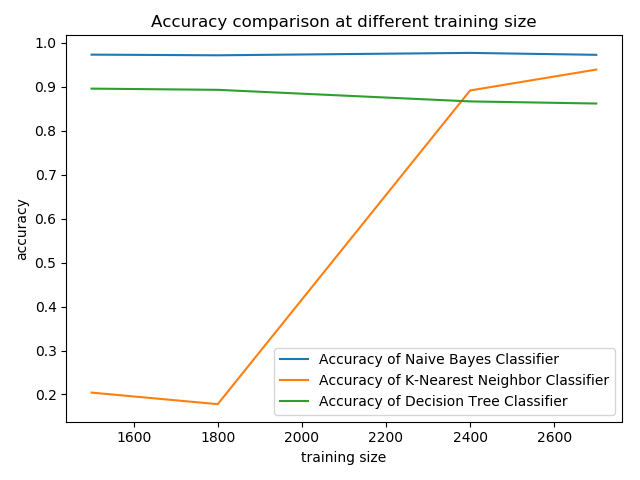
\includegraphics[width=\textwidth]{accuracy_graph.png}
    \caption{Accuracy comparison at different training size}
\end{figure}


We choose four training sets with different sizes $N_\mathrm{training} = [1500, 1800, 2400, 2700]$ to train our three classifiers. We show their prediction performances under the test set with size $N_\mathrm{testing} = [3672, 3372, 2772, 2472]$ correspondingly in Fig 1.

Class imbalance can be a problem in machine learning. To make our model robust, in the data preprocessing phase, we made sure that we used the same size of data for ham and spam by dropping some data. Note that normally we use a large portion of all data for training set. However, in our case, we found that three models could already perform well with a small amount of training data, so we don't need the large portion of the data to train. 

For the K Nearest Neighbor we implemented three metrics $L_{1}$, $L_{2}$ and $L_{\infty}$. In the above graph we used the $L_{2}$ metric. In fact, we found that for this task the choice of metric didn't affect our accuracy after we validated the model with the 3 different metrics. 
We also tested different ``K" values for KNN and found that KNN with K = 3 and 9 gave similar performance.
So we choose K=3 for KNN. 

KNN needs more data to perform well compared with other two models. Our explanation is that, when the training size is small, the so called nearest neighbors of our test data may not be the true ``neighbors" from the same class, hence the accuracy of KNN classifier is low. More data is needed so that KNN can make reasonable prediction based on real neighbors that belongs to the same class.

When the training size increases and we have more data in the space, KNN is able to find the true neighbors of the test data, hence the accuracy of K Nearest Neighbor classifier increases. This can be visualized from the figure. We could see that the performance of Naive Bayes Classifier and Decision Tree Classifier are almost constant while the accuracy of K Nearest Neighbor classifier performs poorly with small data size. 
Another problem of KNN is that we need to select the hyperparameter ``K". It adds additional cost to apply KNN. 

For the decision tree, we set the maximal tree depth to 10. A maximal tree depth is necessary so that it can reduce the overfitting. After performing validation experiments with different maximal tree length, we found that 10 may not be the optimal option since the tree can perform equally well with maximal depth 5 or 6. We still choose 10 here because we want to show the overfitting effect of decision tree. 

With such a maximal depth, we observed some performance drop for decision tree after training with more data. It is understandable since decision tree is prone to overfitting with a deep structure. This makes Naïve Bayes favorable later in this task because in decision tree we need to tune additional hyperparameters. However, in Naïve Bayes, it can perform well without tuning much. 

Lastly, the Naive Bayes classifier is the best among these three classifiers for the email classification task and it performed best with all training data size. It is a simple yet powerful model used in this case. We also don't need to worry about hyperparameters.
This complies to the fact that people in the industry are using Naive Bayes for Spam classification.

\end{document} 
